\documentclass{beamer}

\usepackage[utf8]{inputenc}
\usepackage{default}
\usepackage{listings}
\usepackage{hyperref}

\begin{document}

\author{Kristof Meixner \\ Sebastian Geiger}
\date{6 Mai 2014}
\title{fUML Refactoring with EMF\\\small{Business Informatic Group}}

\begin{frame}
 \maketitle
\end{frame}


\begin{frame}
 \frametitle{Overview}

%TODO: 25 slides


\begin{itemize}
 \item Refactoring Overview
 \item UML Models and Refactoring
 \item fUML Introduction
 \item Complex Example
 \item fUML Refactoring
 \item Semantic Preservation
 \item Refactoring Constraints with OCL
 \item Toolchain
 \item EMF Refactor
\end{itemize}

\end{frame}

\begin{frame}[fragile]
\frametitle{Refactoring Overview}
\begin{itemize}
 \item What is refactoring?
 \begin{itemize}
  \item ``defines a set of program restructuring operations'' that ``preserve the behavior of a program'' \cite{mast:REFOOF}
 \end{itemize}
 \item Why do we need it?
 \begin{itemize}
  \item Increases software and/or model quality
  \item Ensures reusability of components
  \item Supports change management in software lifecycle
 \end{itemize}
 \item Examples: rename class, extract superclass, encapsulate field.
 \item Detailed catalogues with refactorings exist (e.g. \cite{fow99})
\end{itemize}

\end{frame}

\begin{frame}
 \frametitle{Recall - UML}
 \begin{itemize}
  \item Unified Modeling Language (v2.4.1) standardized by Object Management Group \cite{man:UML}
  \item General-purpose modeling language in the field of software engineering (Wikipedia)
  \item Includes different diagram types for architecture structure \& behavior
 \end{itemize}
\begin{figure}[h!t]
 \centering
 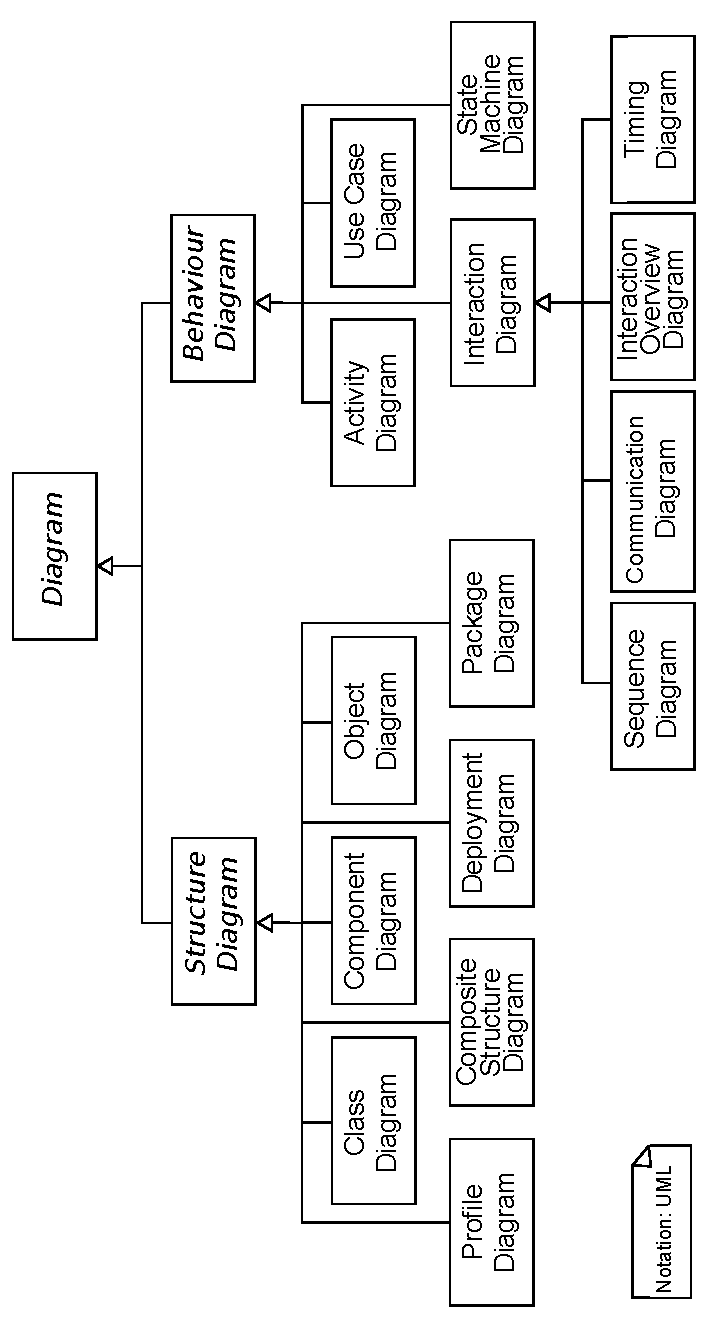
\includegraphics[scale=0.35,angle=270]{images/uml}
 \caption{\textit{UML} diagram type hierarchy (Derfel73, PMerson)}
 \label{fig:uml}
\end{figure}
\end{frame}



\begin{frame}
\frametitle{UML Models and Refactoring}
\begin{itemize}
 \item Whats the difference between source code and model refactoring?
 \begin{itemize}
  \item Consider all interconnected views/diagrams
  \item Consider model constraints
  \item Consider different accuracy levels
 \end{itemize}
 \item How can we preserve behavior/semantics?
 \begin{itemize}
  \item Static analysis of models (e.g. ``code smells'' like complexity or dependencies)
  \item Dynamic analysis of models (e.g. via behavior during execution)
 \end{itemize}
\end{itemize}        
\end{frame}
        
\begin{frame}
\frametitle{fUML Introduction}
\begin{itemize}
 \item fUML = foundational UML
 \item fUML 1.1 is based on UML 2.4.1
 \item Subset of UML (Class and Activity diagrams)
 \item Enhanced with consise semantics
 \item Turing complete and allows execution or interpretation
 \item Existing VM to execute models
 \item Extended VM for testing and debugging (Moliz) \cite{DBLP:conf/models/MayerhoferLK12}
\end{itemize}
\end{frame}

\begin{frame}
\frametitle{fUML Abstract Syntax 1/2}
\begin{figure}[h!t]
 \centering
 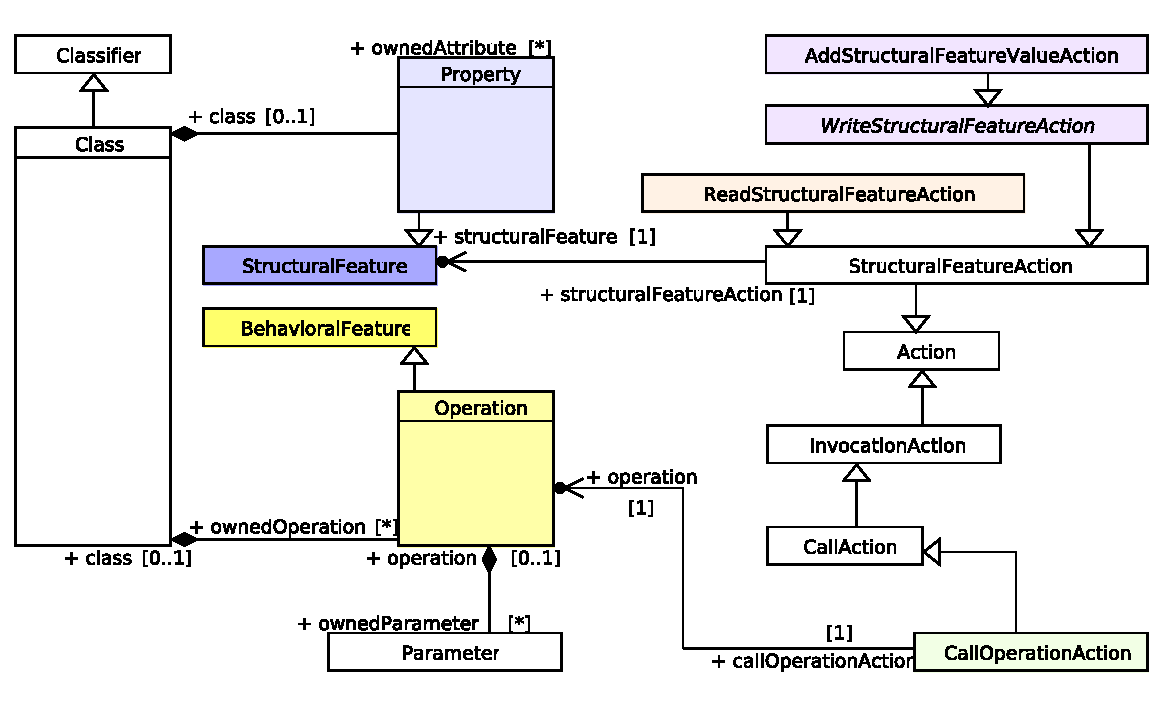
\includegraphics[scale=0.5]{images/Model_Model_Classifiers}
 \caption{Classifiers in fUML}
 \label{fig:classifiers}
\end{figure}
\end{frame}

\begin{frame}
\frametitle{fUML Abstract Syntax 2/2}
\begin{figure}[h!t]
 \centering
 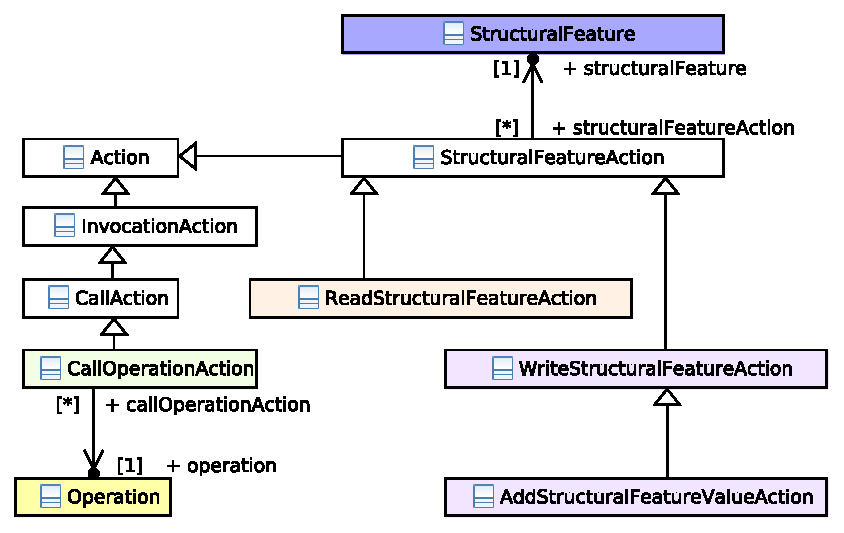
\includegraphics[scale=0.5]{images/Model_Model_Behavior}
 \caption{Actions in fUML}
 \label{fig:behavior}
\end{figure}
\end{frame}

\begin{frame}
\frametitle{Complex Example 1/3}
\begin{figure}[h!t]
 \centering
 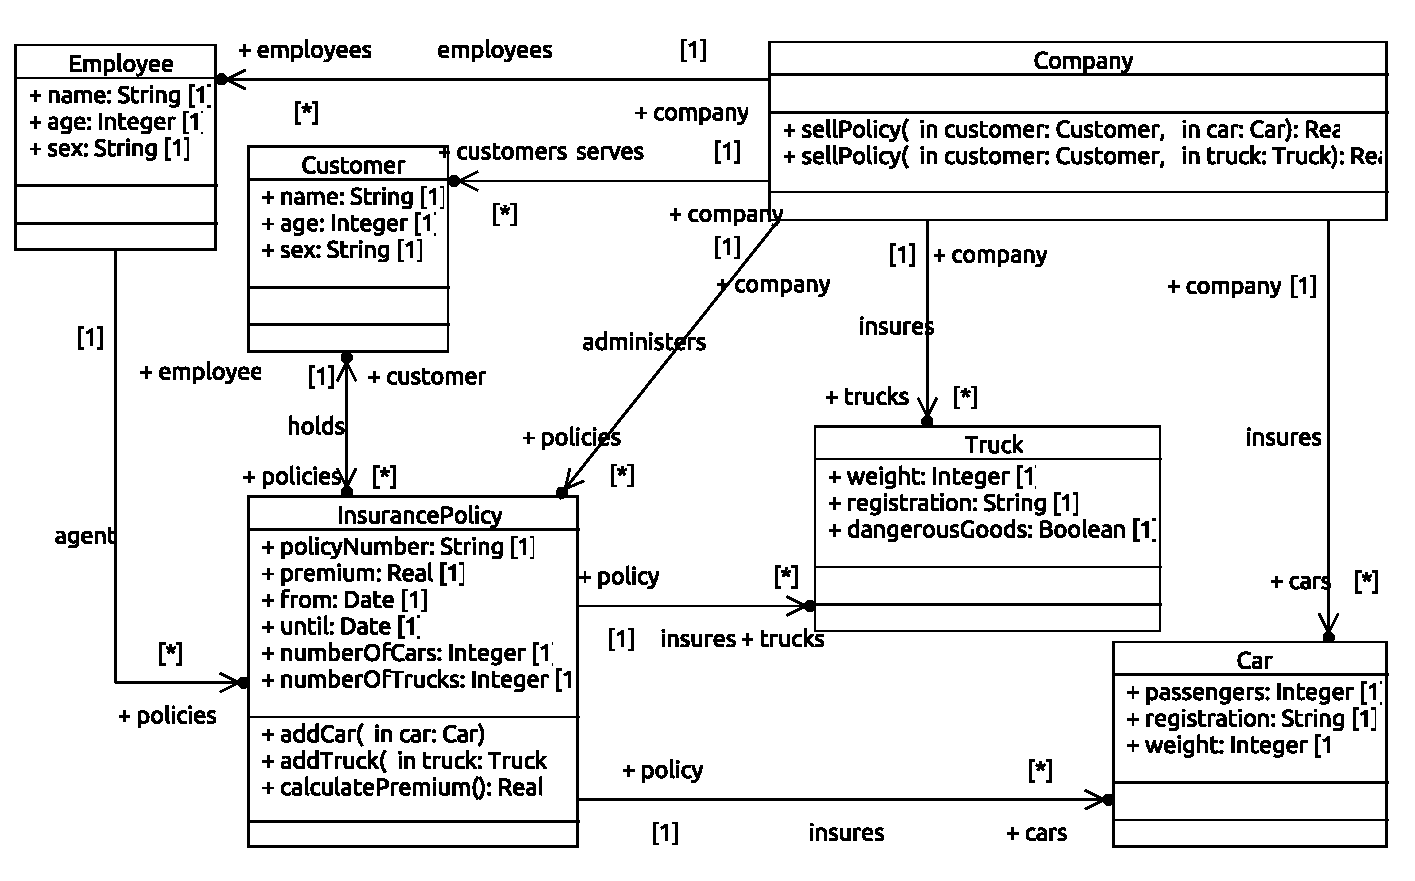
\includegraphics[scale=0.4]{images/insurance/Model_Model_ClassDiagram}
 \caption{Insurance class diagram}
 \label{fig:classdiagramcomplexRef}
\end{figure}
 %\includegraphics{} %TODO: add graphic
\end{frame}

        
\begin{frame}
\frametitle{Complex Example 2/3}
\begin{figure}[h!t]
 \centering
 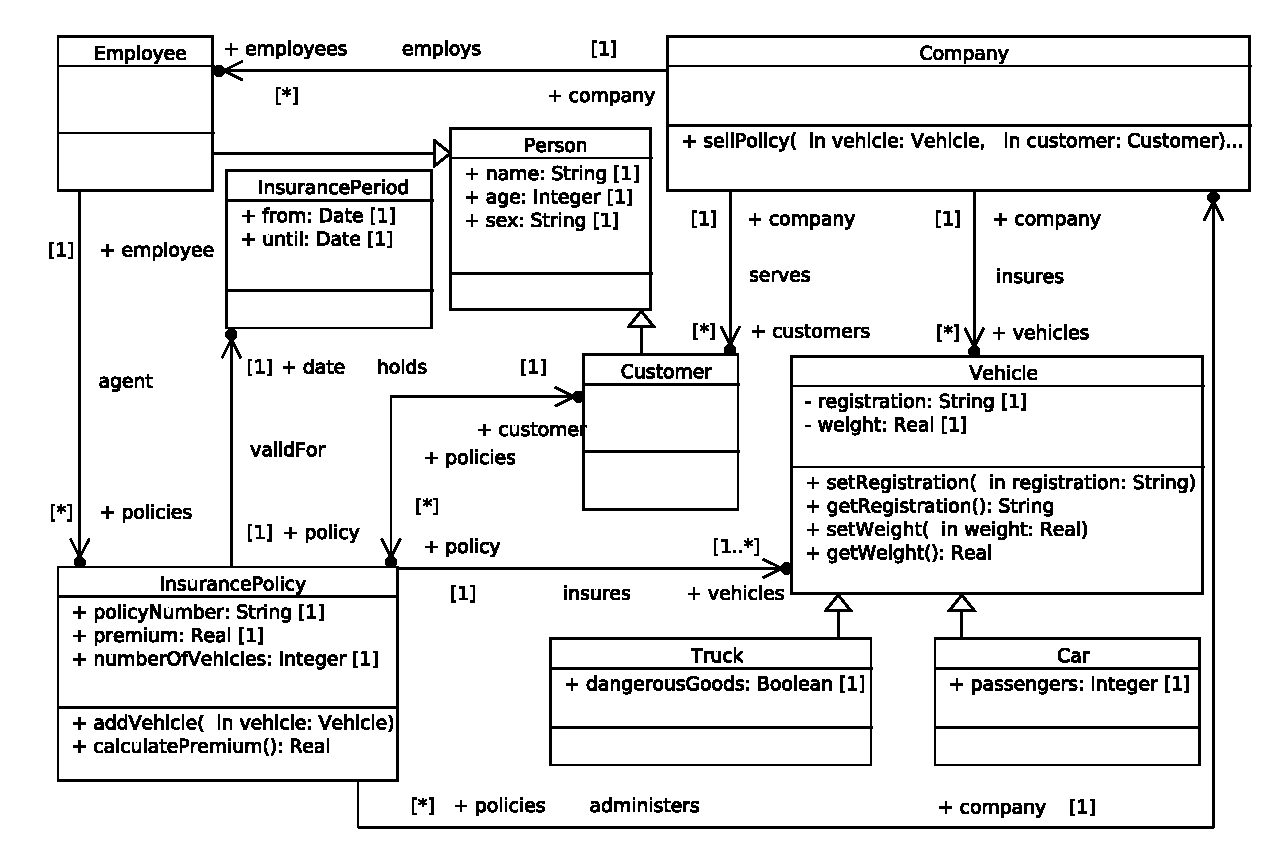
\includegraphics[scale=0.4]{images/insurance_ref/Model_Model_ClassDiagram}
 \caption{Insurance class diagram with refactorings}
 \label{fig:classdiagramcomplex}
\end{figure}
 %\includegraphics{} %TODO: add graphic
\end{frame}

\begin{frame}
\frametitle{Complex Example 3/3}
\begin{figure}[h!t]
 \centering
 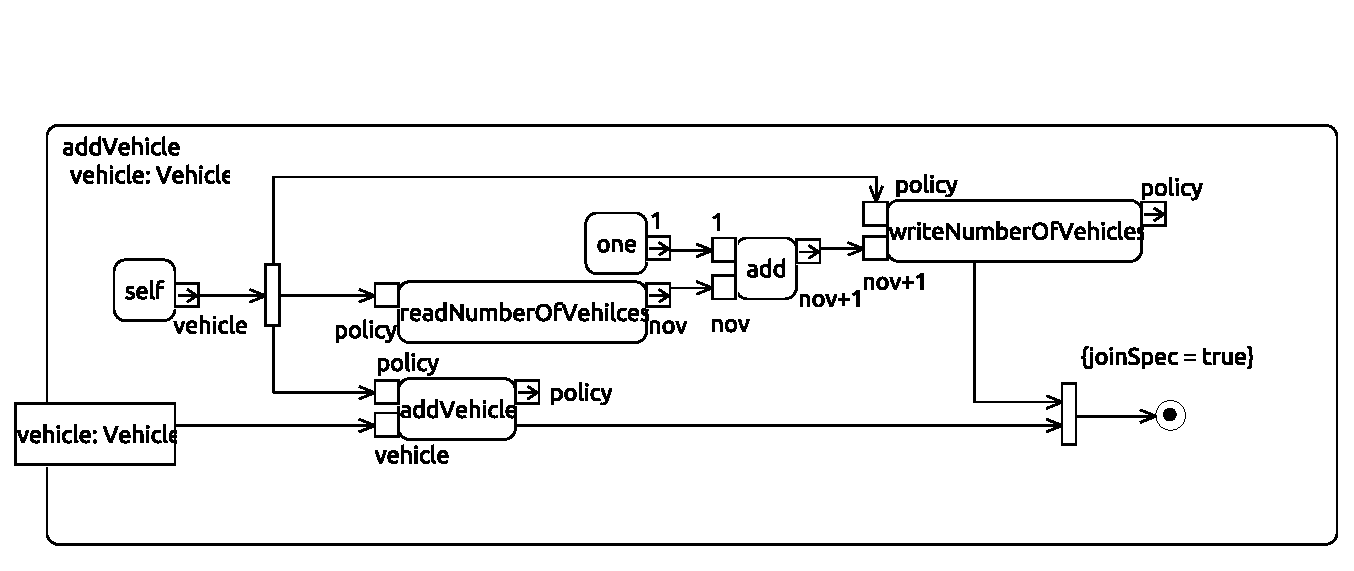
\includegraphics[scale=0.45]{images/insurance_ref/Activity_addVehicle_addVehicle}
 \caption{Add vehicle activity}
 \label{fig:calculatePremium}
\end{figure}
 %\includegraphics{} %TODO: add graphic
\end{frame}

        
%USE 2-3 slides for this!
\begin{frame}
\frametitle{fUML Refactoring}
    \begin{itemize}
     \item Show example of encapsulate field.
    \end{itemize}
\end{frame}
        
\begin{frame}
\frametitle{Semantic Preservation}
\begin{itemize}
 \item What means semantic preservation?
 \begin{itemize}
  \item Same execution trace?
  \item Same output?
  \item Same state?
 \end{itemize}
 \item Depends on refactoring!
 \item How to preserve semantics?
 \begin{itemize}
  \item Specify pre- and postconditions with OCL constraints
  \item Validate refactored models.
  \item Execute models and analyse execution properties (trace).
 \end{itemize}
\end{itemize}

\end{frame}
        
\begin{frame}
\frametitle{Refactoring Constraints with OCL}

\end{frame}
        
\begin{frame}
\frametitle{Toolchain}
        
\end{frame}
        
\begin{frame}
\frametitle{EMF Refactor}
        
\end{frame}
        

\begin{frame}
 \begin{center}
\Huge Questions?
\end{center}
\end{frame}

\begin{frame}
 \frametitle{References}
 \bibliographystyle{acm}
 \bibliography{references}
\end{frame}

\end{document}
